\documentclass[a4paper]{scrartcl}

% font/encoding packages
\usepackage[utf8]{inputenc}
\usepackage[T1]{fontenc}
\usepackage{lmodern}
\usepackage[ngerman]{babel}
\usepackage[ngerman=ngerman-x-latest]{hyphsubst}

\usepackage{amsmath, amssymb, amsfonts, amsthm}
\usepackage{array}
\usepackage{stmaryrd}
\usepackage{marvosym}
\allowdisplaybreaks
\usepackage[output-decimal-marker={,}]{siunitx}
\usepackage[shortlabels]{enumitem}
\usepackage[section]{placeins}
\usepackage{float}
\usepackage{units}
\usepackage{listings}
\usepackage{pgfplots}
\pgfplotsset{compat=1.12}
\usepackage{tikz}
\usetikzlibrary{arrows,automata}

\usepackage{xcolor}
\definecolor{light-gray}{HTML}{cccccc}


\newtheorem*{behaupt}{Behauptung}
\newcommand{\gdw}{\Leftrightarrow}
\newcommand{\dif}{\ \mathrm{d}}
\newcommand{\N}{\mathbb{N}}
\newcommand{\prob}{\mathbb{P}}
\newcommand{\cov}{\operatorname{Cov}}
\newcommand{\e}{\mathbb{E}}
\newcommand{\var}{\operatorname{Var}}
\newcommand{\corr}{\operatorname{Corr}}

\usepackage{fancyhdr}
\pagestyle{fancy}

\lstset{%
    frame=single,
    numbers=left,
    keepspaces,
    language=R,
    title=Listing: \lstname,
}

\def \blattnr {12}

\lhead{Stochastik 2 - Blatt {\blattnr}}
\rhead{Florian Abt, Lennart Braun, Sascha Schulz}
\cfoot{\thepage}


\title{Stochastik 2 für Informatiker}
\subtitle{Blatt {\blattnr} Hausaufgaben}
\author{
    Florian Abt (6524404), \\
    Lennart Braun (6523742), \\
    Sascha Schulz (6434677)
}
\date{zum 19. Januar 2016}
\usepackage{pdfpages} 

\begin{document}
\maketitle

\begin{enumerate}[label=\bfseries \blattnr.\arabic*]
    \item %.1
       Im Fall von k=0.5 scheint die Breite der Konfidenzintervalle bei 
       steigendem n und konstantem Konfidenzniveau monoton zu fallen.
       
       Bei k=1.5 und k=2.5 ist diese Monotonie nur bedingt zu beobachten, es 
       kommt zu Sprungstellen, in denen einzelne (seltene) extreme 
       Werte dazu führen, dass das Konfidenzintervalle sprungartig wieder sehr 
       viel breiter wird.
       

	  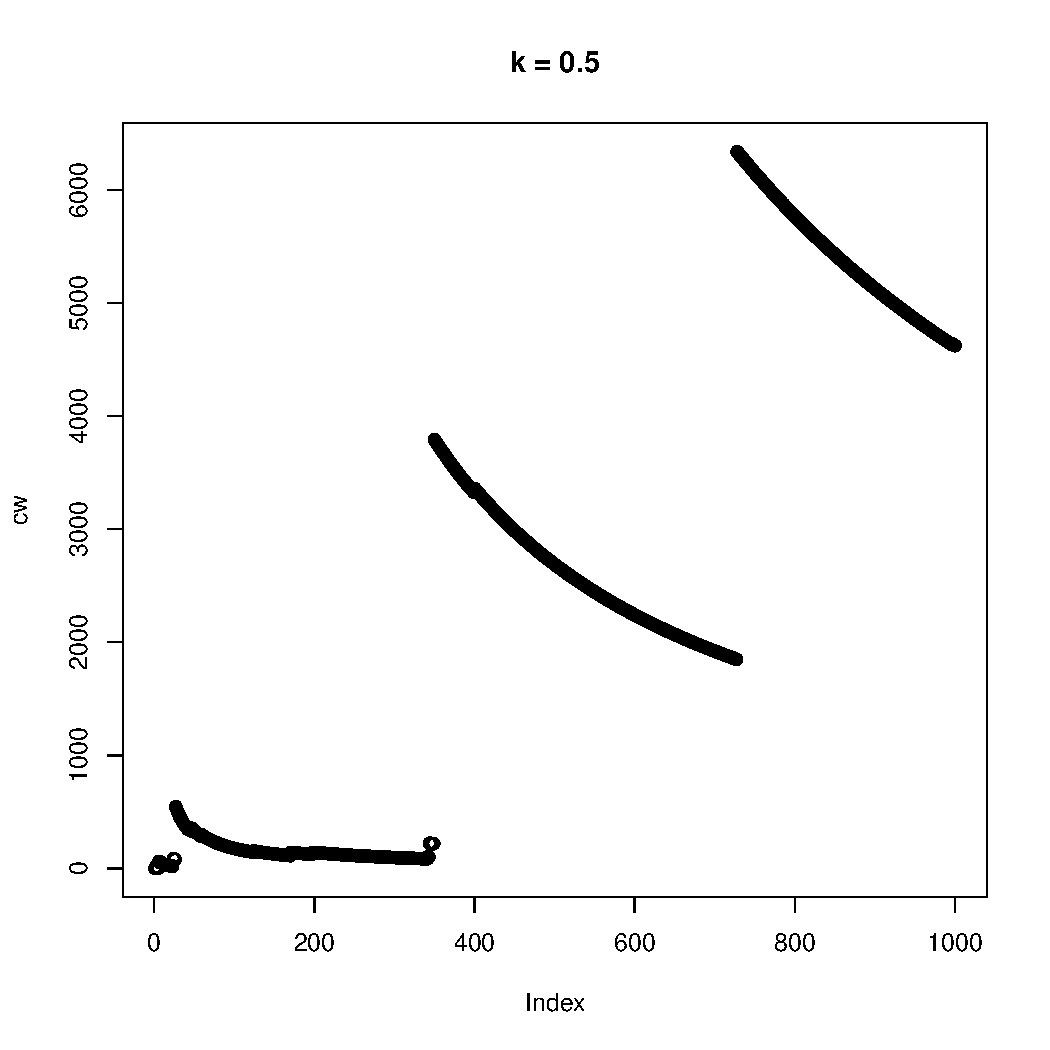
\includegraphics[width=.33\textwidth, page=1]{Rplots.pdf}
	  \includegraphics[width=.33\textwidth, page=2]{Rplots.pdf}
	  \includegraphics[width=.33\textwidth, page=3]{Rplots.pdf}
       
       Anmerkung: Die x-Achse repräsentiert Anzahl der ersten n berücksichtigten 
       Samples mit $2\leq n \leq 1000$, die y-Achse repräsentiert die Breite 
       der Konfidenzintervalle. Die konkrete Darstellung ist stark von der 
       zufälligen Eingabe abhängig, lediglich das oben beschriebene Grundmuster
       lässt sich bei wiederholter Ausführung erkennen.

    \item %.2
        \begin{enumerate}
            \item
              Die Inversionsmethode kann angewendet werden, da die $U_i$ iid auf 
              [0,1) und gleichverteilt sind. Außerdem ist F rechtsseitig stetig 
              sodass stets \\ 
              $\mathbb{P}(U\leq F(x))=F(x)$.
              
	      \begin{equation*}
		F^{-1}(y) = \begin{cases}
			      1 &, y \in \left[0,\frac16 \right) \\
			      2 &, y \in \left[\frac16, \frac26 \right)\\
			      3 &, y \in \left[\frac26,\frac36 \right)\\
			      4 &, y \in \left[\frac36,\frac46 \right)\\
			      5 &, y \in \left[\frac46,\frac56 \right)\\
			      6 &, y \in \left[\frac56,1 \right)
		            \end{cases}
	      \end{equation*}
	      
            \item
	      \begin{tabular}{c|c|c|c|c|c}
	       $i$ & 1 & 2 & 3 & 4 & 5 \\
	       \hline
	       $u_i$ & 0.1 & 0.32 & 0.88 & 0.02 & 0.7 \\
	       \hline
	       $x_i$ & 1 & 2 & 9 & 1 & 8
	      \end{tabular}

            \item

        \end{enumerate}

    \item %.3
        \begin{enumerate}
            \item

            \item

            \item

        \end{enumerate}

\end{enumerate}

\end{document}

